\documentclass{article}
\usepackage{amsmath}
\usepackage[margin=1.2in]{geometry}
\usepackage{graphicx} 
\usepackage{float}

\title{Kalman Filter for Quadcopter Position Hold}
\author{Peter Davidson and Pantelis Sopasakis}


\begin{document}
\maketitle

\section{Problem statement}
The system dynamics is described by Newton's second law of motion.
Let $z$ be the altitude of the quadcopter, $g$ denotes the acceleration
due to gravity and $a$ is the acceleration that results from the forces
of the propellers. Then, the system dynamics is as simple as
\begin{equation}
    \ddot{z} = a - g.
\end{equation}
The acceleration, $a$, is an affine function of the thrust reference signal
(which comes from the RC); it is
\begin{eqnarray}
    a = \alpha \tau + \beta,
\end{eqnarray}
where $\alpha$ and $\beta$ are coefficients to be estimated; we can obtain
\textit{a priori} estimates offline and update them online using measurements
while flying (using the Kalman filter).


@Peter,
\begin{enumerate}
    \item Copy here the system dynamics from Chandra's report (we don't need Section 2.2.3)
    \item Write down what sensors we use and what their characteristics are (level of noise,
          presence of outliers, whether the sensors are biased, update frequencies)
\end{enumerate}
and we'll take it from there.

% \section{Introduction}
% In this section, we delve into the application of Kalman filters for sensor fusion in quadcopter navigation, integrating data from GNSS modules, barometers, and time-of-flight sensors. The Kalman filter, a powerful algorithm for linear dynamic systems, it excels in estimating the state of a process by minimizing the mean squared error. It operates in two phases: prediction and update. During the prediction phase, it projects the current state and uncertainty forward in time. Then, in the update phase, it adjusts the projected estimate by incorporating new measurements, thereby refining the accuracy. By leveraging the Kalman filter, our aim is to enhance positioning accuracy and reliability, utilizing the unique advantages of each sensor to achieve a cohesive and robust solution for improved quadcopter control and stability for postition hold.

% \section{Prediction phase}
% The prediction phase of the Kalman filter forecasts the system's future state by extrapolating current estimates using system dynamics. It predicts the quadcopter's next position and velocity, incorporating uncertainties and process noise to account for potential deviations. This step ensures continuous trajectory estimation, crucial for real-time navigation adjustments.
% \\

% \noindent
% The state prediction phase is fundamental to forecasting the system's future state based on its current status and inherent dynamics. This phase is comprised of two main components:

% \subsection{State Prediction}
% The future state, denoted as \( \widetilde{x}_{t+1} \), is predicted by applying the State Transition Matrix, \( A_t \), to the current estimated state, \( \widetilde{x}_t \), assuming the expected value of the process noise, \( w_t \), is zero. The prediction is thus given by:
% \[
% \widetilde{x}_{t+1} = A_t \widetilde{x}_t
% \]
% This equation reflects the natural progression of the system from one state to the next, devoid of external inputs.

% \subsection{Estimated Variance Prediction}
% The variance of the estimator for the next state, \( P_{t+1} \), is also predicted to represent the uncertainty in the state estimate. This prediction incorporates the Process Noise Covariance Matrix, \( Q_t \), and is expressed as:
% \[
% P_{t+1} = A_t P_t A_t^T + G_t Q_t G_t^T
% \]
% Here, \( G_t \) adjusts the process noise to the state space dimensions, and \( A_t \) forwards the current error covariance in time.
% \\

% \noindent
% These predictive steps ensure the Kalman Filter has a baseline forecast of the system's state, which is then refined with incoming measurements during the update phase, maintaining the filter's accuracy and reliability.

% \section{Update phase}

% The update phase incorporates the latest measurements to refine the state estimates. The key equations involved in this phase are as follows:


% \subsection{Kalman Gain Calculation}
% Calculate the Kalman Gain \( K_t \), which dictates the extent to which the predicted state is corrected based on the measurement:
% \[ K_t = P_{t} C^T (C_t P_t C^T + R)^{-1} \]
% where \( R_t \) is the measurement noise covariance matrix.

% \subsection{State Update}
% Update the state estimate with the new measurement by applying the Kalman Gain to the innovation:
% \[ \widetilde{x}_{t+1} = \widetilde{x}_{t} + K_t ( y_t + - C\widetilde{x}_t)\]

% \subsection{Covariance Update}
% Update the estimate's error covariance to reflect the decrease in uncertainty:
% \[ P_{t+1} = (I - K_t C) P_{t} \]
% where \( I \) is the identity matrix.


\newpage
\section{Altitude Dynamics}
The altitude dynamics of a quadcopter are defined within a global coordinate system, crucial for maintaining a predetermined altitude from the Earth's surface. The model that describes these dynamics is based on fundamental principles, delineated as follows:

The rate of change of the quadcopter's altitude, represented as \( \dot{z}_t \), is the result of the vertical acceleration \( a^z_{T_t} \) produced by the drone's motors at a given time minus the gravitational acceleration, \( g \). This equation is continuous in time and is expressed as,
\begin{equation}
\dot{z}_t = a^z_{T,t} - g
\end{equation}
\noindent
Here, \( a^z_{T_t} \) signifies the upward acceleration generated by the propulsion at time \( t \), measured in meters per second squared. The constant \( g \) denotes the acceleration due to Earth's gravity, also in meters per second squared. The altitude \( z_t \) represents the drone's center of mass's vertical position at time \( t \), measured in meters.

Additionally, the drone's vertical velocity \( v_{z_t} \) and vertical acceleration \( a_{z_t} \) are defined by the rate of altitude change \( \dot{z}_t \) and the rate of vertical acceleration change \( \dot{a}^z_{T_t} - g \), respectively. The term \( \dot{a}^z_{T_t} \) is derived from the quadcopter's upward thrust and serves as the system's input, while \( g \) is considered a constant input in the opposite direction.

Let \( y_{t}^z = z_t \) be the output equation of the system. Then the corresponding state-space representation is,
\begin{equation}
\begin{bmatrix}
v_{v,t}\\
a_{t}^z
\end{bmatrix} =
\begin{bmatrix}
0 & 1 \\
0 & 0 
\end{bmatrix}
\begin{bmatrix}
z\\
v_{v,t}
\end{bmatrix} + 
\begin{bmatrix}
0 & 0 \\
1 & 1 \\ 
\end{bmatrix}
\begin{bmatrix}
a_{T,t}^z \\ 
-g
\end{bmatrix},\label{eq:4}
\end{equation}

\noindent
for the barometer sensor's output, denoted by \( y_{barom} \), is described by the equation,
\begin{equation}
y_{barom} = z + d^{bar} + e_{barom}
\end{equation}

where, 
\begin{equation}
    d^{bar}_{t+1} = d^{bar}_t + w_{t}^{d^{bar}}
\end{equation}
The bias $(d^{bar})$ should stay consistent throughout readings, 
the second reading of the bias should be equal to the first allowing for some additional noise/offest.

\noindent
for the GPS sensor's output, denoted by \( y_{gps} \), is described by the equation,
\begin{equation}
y_{gps} = z + e_{gps}
\end{equation}

\begin{equation}
y_{gps} =
\begin{bmatrix}
    1 & 0
\end{bmatrix}
x + e_{gps}
\end{equation}

\noindent
The Time-of-Flight (ToF) sensor's output, denoted by \( y_{ToF} \), is described by the equation,
\begin{equation}
y_{ToF} = z + d^{tof} + e_{ToF}
\end{equation}

\noindent
Throught all sensors \( y \) represents the output from the sensor. The variable \( z \) signifies the quadcopter's altitude, which is the measurement for all sensors. The term \( e \) encapsulates the measurement noise or errors associated with the sensors. This noise term, \( e \), encompasses various factors such as sensor inaccuracies, the impact of environmental conditions on sensor performance, and any systematic bias that might be inherent in the sensor's readings.

\noindent
Equation \eqref{eq:4} describes the continuous-time altitude dynamics of the quadcopter. The dis-
cretization of the altitude dynamics of the system (2) with a sampling frequency of Ts using the zero-order hold technique is,

\begin{equation}
\begin{bmatrix}
z_{t+1}\\
v_{z,t+1}
\end{bmatrix} =
\begin{bmatrix}
1 & T_s \\
0 & 1 
\end{bmatrix}
\begin{bmatrix}
z_t\\
v_{s,t}
\end{bmatrix} + 
\begin{bmatrix}
{1/2}{T^2}_s & {1/2}{T^2}_s \\
T_s & T_s \\ 
\end{bmatrix}
\begin{bmatrix}
a_{T,t}^z \\ 
-g
\end{bmatrix},
\end{equation}
\subsection{State Vector Definition}
The state vector \( x_t \) is defined as,
\[
    x_t = 
    \begin{bmatrix}
        z_t &
        e_{t} & 
        \alpha_t & 
        \beta_t &
        d^{bar}_t 
    \end{bmatrix}
\]

\subsection{State Transition Equation}
\begin{equation}
    {x}_{t+1} = A_t {x}_t + W_t
\end{equation}

\subsection{Measurement Model}
The measurement model is defined as,
\begin{equation}
y_t = C_t x_t + e_t
\end{equation}
\begin{equation}
    y_t  = 
    \begin{bmatrix}
        1 & 0 & 0 & 0 & 0 \\
        1 & 0 & 0 & 0 & 0 \\
        1 & 0 & 0 & 0 & 1 \\
    \end{bmatrix}
        x_t + e_t
\end{equation}

\section{Estimator Design}
\begin{align}
    z_{t+1} =& z_t + T_s v_t^z + \frac{1}{2} T_s^2 (\alpha_t \tau_t + \beta_t) + w_t^z\\
    v_{t+1}^z =& v_t^z + T_s (\alpha_t \tau_t + \beta_t) + w_t^v,\\
    \alpha_{t+1} =& \alpha_t + w_t^\alpha,\\
    \beta_{t+1} =& \beta_t + w_t^\beta\\
\end{align}
\noindent
We define $w_t^z$ and $w_t^v$ as the process noise elements.
$w_t^z$ is distributed normally with zero mean and variance
$\sigma_z^2$, expressed as $w_t^z \sim \mathcal{N}(0, \sigma_z^2)$, 
and similarly, $w_t^v$ follows a normal distribution with $w_t^v \sim \mathcal{N}(0, \sigma_v^2)$.
Additionally, $w_t^\alpha$ and $w_t^\beta$ represent white noise processes with distributions
$w_t^\alpha \sim \mathcal{N}(0, T_s \sigma_\alpha^2)$ and $w_t^\beta \sim \mathcal{N}(0, T_s \sigma_\beta^2)$ 
respectively. The system's state needing estimation is denoted by $x_t = (z_t, v_t^z, \alpha_t, \beta_t)$, 
with the system's dynamic model being describable as follows,
\begin{equation}
    x_{t+1} = A_t x_t + w_t^z,
\end{equation}

where the matrix $A_t$ is defined as,
\begin{equation}
    A_t = 
    \begin{bmatrix}
    1 & T_s & \frac{1}{2} T_s^2 \tau_t & \frac{1}{2} T_s^2 \\
    0 & 1 & T_s \tau_t & T_s \\
    0 & 0 & 1 & 0 \\
    0 & 0 & 0 & 1
    \end{bmatrix}
\end{equation}

altitude:
\begin{equation}
    Z_{t+1} = Z_t + {T_s}{V_t} + {w^z}_t
\end{equation}

velocity:
\begin{equation}
    V_{t+1} = V_t + T_s({\alpha_t}{\tau_t} + \beta_t) + {w^v}_t
\end{equation}
where, 
\begin{equation}
    a_t =
    {\alpha_t}{\tau_t} + \beta_t
\end{equation}

\section{Relationship between thrust and lift}
\begin{figure}[H]
    \centering
    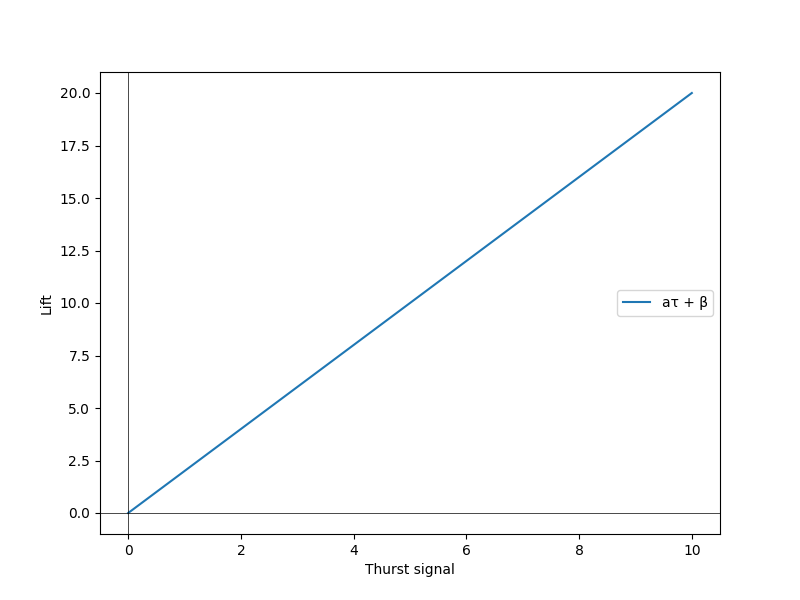
\includegraphics[width=0.5\textwidth]{Figure_1.png}
    \label{fig:fig1}
    \caption{}
\end{figure}
This graph represents the relationship between throttle signal 
From our radio, and how this effects the lifing force on the quad.
(please note that this graph is not to scale)
This relationship is catagorised by the equation, 
\[
\alpha_t\tau_t + \beta_t
\]

\end{document}